%% ============================================================
%% NN-POLAN: Physics-Informed Neural Network Ionogram Inversion
%% Show-and-Tell Presentation — Beamer
%%
%% Compile:
%%   cd tutorials/nn_inv
%%   pdflatex nn_inversion_ppt.tex && pdflatex nn_inversion_ppt.tex
%%
%% Or via project root:
%%   make tutorials-nn-ppt
%% ============================================================
\documentclass[aspectratio=169,10pt]{beamer}

% ---------- theme ------------------------------------------------
\usetheme{Madrid}
\usecolortheme{crane}
\setbeamertemplate{navigation symbols}{}
\setbeamertemplate{footline}[frame number]
\setbeamerfont{frametitle}{size=\normalsize,series=\bfseries}
\setbeamercolor{block title}{bg=blue!15,fg=blue!60!black}
\setbeamercolor{block body}{bg=blue!5}
\setbeamercolor{alertblock title}{bg=orange!25,fg=orange!70!black}
\setbeamercolor{alertblock body}{bg=orange!5}
\setbeamercolor{exampleblock title}{bg=green!15,fg=green!50!black}
\setbeamercolor{exampleblock body}{bg=green!5}

% ---------- packages ------------------------------------------------
\usepackage{amsmath,amssymb}
\usepackage{graphicx}
\usepackage{listings}
\usepackage{xcolor}
\usepackage{booktabs}
\usepackage{hyperref}
\usepackage{tikz}
\usepackage{multirow}
\usepackage{colortbl}
\usepackage{array}
\usetikzlibrary{arrows.meta,positioning,shapes,fit,backgrounds,
                decorations.pathreplacing,calc,matrix}

% ---------- code style ------------------------------------------------
\definecolor{codebg}{RGB}{245,245,250}
\definecolor{codekw}{RGB}{0,0,180}
\definecolor{codestr}{RGB}{160,32,32}
\definecolor{codecom}{RGB}{0,128,0}

\lstset{
  language=Python,
  backgroundcolor=\color{codebg},
  basicstyle=\ttfamily\tiny,
  keywordstyle=\color{codekw}\bfseries,
  stringstyle=\color{codestr},
  commentstyle=\color{codecom}\itshape,
  showstringspaces=false,
  breaklines=true,
  frame=single,framerule=0.4pt,
  rulecolor=\color{gray!40},
  xleftmargin=2pt,xrightmargin=2pt,
}

% ---------- tikz styles ------------------------------------------------
\tikzset{
  box/.style={draw,rounded corners=2pt,align=center,font=\tiny,
              minimum width=1.8cm,minimum height=0.48cm},
  arr/.style={-{Stealth[length=4pt]},thick},
  pbox/.style={box,fill=blue!12},
  obox/.style={box,fill=orange!15},
  gbox/.style={box,fill=green!12},
  rbox/.style={box,fill=red!10},
  ybox/.style={box,fill=yellow!18},
  grbox/.style={box,fill=gray!10},
  filmbox/.style={box,fill=yellow!30,draw=orange!60,thick},
  blk/.style={draw,rounded corners=2pt,align=center,font=\tiny,
              fill=blue!10,minimum width=2.8cm,minimum height=0.55cm},
  oblk/.style={blk,fill=orange!12},
}

% ---------- title info -----------------------------------------------
\title[NN-POLAN — Show \& Tell]{%
  \textbf{NN-POLAN}: Physics-Informed Neural Network\\
  Ionogram Inversion}
\subtitle{Architecture · Training · Validation · Sporadic-E Extension}
\author{S. Chakraborty \textit{et al.}}
\institute{Embry-Riddle Aeronautical University \;|\; pynasonde project}
\date{\today}

% =================================================================
\begin{document}
% =================================================================

\begin{frame}
  \titlepage
  \vspace{-0.4cm}
  \begin{center}
    \scriptsize
    \texttt{pynasonde.vipir.analysis.nn\_inversion}\quad|\quad
    \href{https://github.com/shibaji7/pynasonde}{github.com/shibaji7/pynasonde}
  \end{center}
\end{frame}

% \begin{frame}{Outline}
%   \tableofcontents
% \end{frame}

% =================================================================
\section{Motivation}
% =================================================================

\begin{frame}{The Ionogram Inversion Problem}
\begin{columns}
\column{0.54\textwidth}
  \begin{block}{What we measure vs.\ what we want}
    \small
    \textbf{Measure}: virtual-height trace $h'(f)$ — apparent reflection height\\
    \textbf{Want}: true electron density profile $N(h)$
  \end{block}
  \vspace{3pt}
  \textbf{Abel integral} (forward model):
  \[
    h'(f) = h_0 + \int_{h_0}^{h_r(f)} \frac{dh}{\sqrt{1 - f_p^2(h)/f^2}}
  \]
  where $f_p = \sqrt{N_e/12441}\,[\text{MHz}]$ is the plasma frequency.\\[4pt]
  \textbf{Inversion} = find $N(h)$ such that Abel($N$) $= h'(f)$\\
  Classical solver: \textbf{POLAN} (iterative, ~1--5 s/ionogram)

\column{0.43\textwidth}
  \begin{alertblock}{POLAN limitations}
    \scriptsize
    \begin{itemize}
      \item[$\times$] Sequential, slow per ionogram
      \item[$\times$] Requires clean, scaled traces
      \item[$\times$] Fails on spread-F, oblique echoes
      \item[$\times$] No uncertainty estimate
    \end{itemize}
  \end{alertblock}
  \vspace{3pt}
  \begin{exampleblock}{NN-POLAN targets}
    \scriptsize
    \begin{itemize}
      \item[$\checkmark$] $<$1 ms/ionogram (GPU batch)
      \item[$\checkmark$] Works on raw/noisy traces
      \item[$\checkmark$] Physics-constrained via Abel loss
      \item[$\checkmark$] Generalises across stations \& seasons
    \end{itemize}
  \end{exampleblock}
\end{columns}
\end{frame}

% =================================================================
\section{Data Pipeline}
% =================================================================

\begin{frame}{Synthetic Data Generation Pipeline}
\vspace{-0.15cm}
\begin{center}
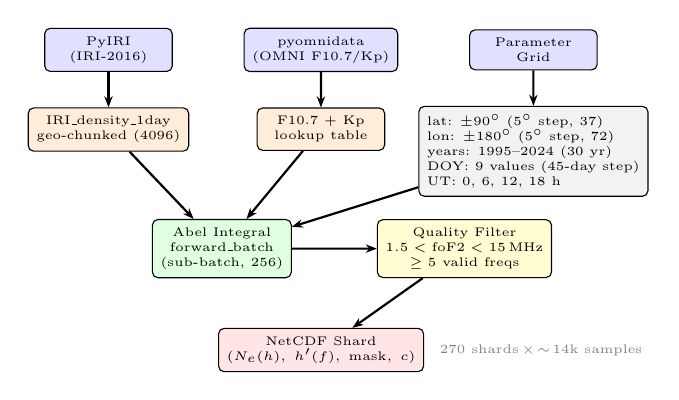
\begin{tikzpicture}[>=Stealth,node distance=0.38cm and 0.65cm,
                    every node/.style={font=\tiny},scale=0.90,transform shape]

\node[pbox] (pyiri)  {PyIRI\\(IRI-2016)};
\node[pbox,right=1.0cm of pyiri] (omni)  {pyomnidata\\(OMNI F10.7/Kp)};
\node[pbox,right=1.0cm of omni]  (grid)  {Parameter\\Grid};

\node[grbox,below=0.5cm of grid,minimum width=2.4cm,align=left] (gridbox) {
  lat: $\pm90^{\circ}$ (5$^{\circ}$ step, 37)\\
  lon: $\pm180^{\circ}$ (5$^{\circ}$ step, 72)\\
  years: 1995--2024 (30 yr)\\
  DOY: 9 values (45-day step)\\
  UT: 0, 6, 12, 18 h
};

\node[obox,below=0.5cm of pyiri]  (batch) {IRI\_density\_1day\\geo-chunked (4096)};
\node[obox,below=0.5cm of omni]   (sw)    {F10.7 + Kp\\lookup table};

\node[gbox,below=0.95cm of batch,xshift=1.6cm] (fwd)
  {Abel Integral\\forward\_batch\\(sub-batch, 256)};
\node[ybox,right=1.2cm of fwd] (qc)
  {Quality Filter\\$1.5 < \mathrm{foF2} < 15$\,MHz\\$\geq 5$ valid freqs};
\node[rbox,below=0.7cm of fwd,xshift=1.4cm] (nc)
  {NetCDF Shard\\$(N_e(h),\;h'(f),\;\text{mask},\;c)$};

\draw[arr] (pyiri) -- (batch);
\draw[arr] (omni)  -- (sw);
\draw[arr] (grid)  -- (gridbox);
\draw[arr] (gridbox) -- (fwd);
\draw[arr] (batch) -- (fwd);
\draw[arr] (sw)    -- (fwd);
\draw[arr] (fwd)   -- (qc);
\draw[arr] (qc)    -- (nc);
\node[font=\tiny,text=gray,right=0.1cm of nc] {270 shards\\\,$\times\!\sim\!14$k samples};
\end{tikzpicture}
\end{center}
\vspace{-2pt}
\begin{columns}
\column{0.50\textwidth}
  \begin{block}{\scriptsize Conditioning vector $c$ (6 values)}
    \scriptsize
    $[\,\mathrm{lat},\;\mathrm{lon},\;\mathrm{DOY},\;\mathrm{UT},\;\mathrm{Kp},\;\mathrm{F10.7}\,]$\quad
    Real solar flux from OMNI; Kp derived from hourly SymH
  \end{block}
\column{0.47\textwidth}
  \begin{block}{\scriptsize Grid specs}
    \scriptsize
    \textbf{Height}: 60--511.5 km, 0.5 km step $\to$ \textbf{904} pts\\
    \textbf{Freq}: 1.0--15.0 MHz, 0.1 MHz step $\to$ \textbf{141} pts
  \end{block}
\end{columns}
\end{frame}

% =================================================================
\section{Architecture}
% =================================================================

\begin{frame}{NNPolan Architecture — Overview}
\begin{columns}
\column{0.58\textwidth}
\vspace{-0.2cm}
\begin{center}
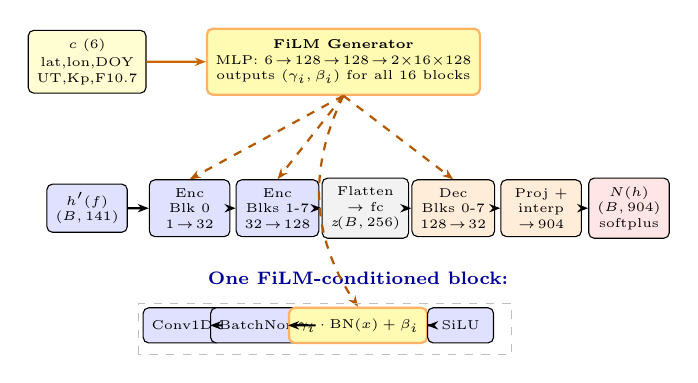
\begin{tikzpicture}[>=Stealth,every node/.style={font=\tiny},
                    node distance=0.3cm and 0.2cm,
                    scale=0.93,transform shape]

%% ---------- conditioning path (top) ----------
\node[filmbox,minimum width=3.6cm,minimum height=0.9cm]
  (film) at (3.5,3.8) {
    \textbf{FiLM Generator}\\
    MLP: $6\!\to\!128\!\to\!128\!\to\!2{\times}16{\times}128$\\
    outputs $(\gamma_i,\beta_i)$ for all 16 blocks
  };

\node[ybox,minimum width=1.3cm] (cin) at (0,3.8)
  {$c$ (6)\\[1pt]\tiny lat,lon,DOY\\UT,Kp,F10.7};
\draw[arr,orange!80!black,thick] (cin) -- (film);

%% ---------- encoder ----------
\node[pbox,minimum width=1.0cm] (inp) at (0,1.8)
  {$h'(f)$\\$(B,141)$};

\node[pbox,minimum width=1.1cm] (e1) at (1.4,1.8)
  {Enc\\Blk 0\\$1\!\to\!32$};
\node[pbox,minimum width=1.1cm] (e2) at (2.6,1.8)
  {Enc\\Blks 1-7\\$32\!\to\!128$};
\node[grbox,minimum width=1.1cm] (lat) at (3.8,1.8)
  {Flatten\\$\to$ fc\\$z\!(B,256)$};

%% ---------- decoder ----------
\node[obox,minimum width=1.1cm] (d1) at (5.0,1.8)
  {Dec\\Blks 0-7\\$128\!\to\!32$};
\node[obox,minimum width=1.1cm] (d2) at (6.2,1.8)
  {Proj +\\interp\\$\to\!904$};
\node[rbox,minimum width=1.1cm] (out) at (7.4,1.8)
  {$N(h)$\\$(B,904)$\\softplus};

%% main flow arrows
\draw[arr] (inp) -- (e1);
\draw[arr] (e1)  -- (e2);
\draw[arr] (e2)  -- (lat);
\draw[arr] (lat) -- (d1);
\draw[arr] (d1)  -- (d2);
\draw[arr] (d2)  -- (out);

%% FiLM injection arrows
\draw[arr,dashed,orange!70!black] (film.south) -- (e1.north);
\draw[arr,dashed,orange!70!black] (film.south) -- (e2.north);
\draw[arr,dashed,orange!70!black] (film.south) -- (d1.north);

%% ---------- FiLM block detail (bottom) ----------
\node[font=\scriptsize\bfseries,text=blue!60!black] at (3.7,0.85)
  {One FiLM-conditioned block:};

\node[pbox,minimum width=0.9cm] (b1) at (1.3,0.2) {Conv1D};
\node[pbox,minimum width=0.9cm] (b2) at (2.4,0.2) {BatchNorm};
\node[filmbox,minimum width=1.4cm] (b3) at (3.7,0.2)
  {$\gamma_i \cdot \mathrm{BN}(x) + \beta_i$};
\node[pbox,minimum width=0.9cm] (b4) at (5.1,0.2) {SiLU};
\draw[arr] (b1)--(b2); \draw[arr] (b2)--(b3); \draw[arr] (b3)--(b4);
\draw[arr,dashed,orange!70!black] (film.south) to[bend right=30] (b3.north);

\draw[gray!50,dashed] (0.7,-0.2) rectangle (5.8,0.5);
\end{tikzpicture}
\end{center}

\column{0.39\textwidth}
\begin{block}{\scriptsize Key specifications}
  \scriptsize
  \begin{tabular}{@{}ll@{}}
  \toprule
  \textbf{Component} & \textbf{Details}\\
  \midrule
  Input & $h'(f)$: $(B,1,141)$\\
  Encoder & 8 Conv1D blocks\\
  Channels & $1\!\to\!32\!\to\!64\!\to\!128$\\
  Stride-2 & 4 of 8 blocks ($141\!\to\!9$)\\
  Bottleneck & flatten$(B,128,9)\!\to\!(B,1152)$\\
  Latent $z$ & $(B, 256)$ via fc 1152$\to$256\\
  Decoder & 8 TConv blocks\\
  Upsamp. & $9\!\to\!18\!\to\!\cdots\!\to\!144$\\
  Final & interp to 904 pts\\
  Output & softplus $\geq 0$\\
  \midrule
  FiLM MLP & $6\!\to\!128\!\to\!128$\\
  FiLM out & $(\gamma_i,\beta_i)$ per block\\
  \midrule
  \textbf{Total params} & \textbf{1.43 M}\\
  \bottomrule
  \end{tabular}
\end{block}
\begin{exampleblock}{\scriptsize Why FiLM conditioning?}
  \scriptsize
  A \emph{single} model covers all:\\
  latitudes, seasons, solar activity,\\
  and local times via $c\!=\!(\gamma,\beta)$
\end{exampleblock}
\end{columns}
\end{frame}

%% -----------------------------------------------------------
\begin{frame}{Architecture — Component Details}
\begin{columns}
\column{0.48\textwidth}

\begin{block}{Encoder (8 Conv1D blocks)}
  \scriptsize
  \textbf{Purpose}: compress $h'(f)$ into a latent representation\\[3pt]
  \begin{tabular}{@{}clcc@{}}
  \toprule
  Blk & Operation & Ch & Stride\\
  \midrule
  0 & Conv1D $k=7$, pad=3 & $1\!\to\!32$  & 1\\
  1 & Conv1D $k=5$, pad=2 & $32\!\to\!32$ & 1\\
  2 & Conv1D $k=5$, pad=2 & $32\!\to\!64$ & 2\\
  3 & Conv1D $k=3$, pad=1 & $64\!\to\!64$ & 1\\
  4 & Conv1D $k=3$, pad=1 & $64\!\to\!128$& 2\\
  5--7 & Conv1D $k=3$, pad=1 & $128\!\to\!128$& 1 or 2\\
  \bottomrule
  \end{tabular}\\[3pt]
  Each block: Conv1D $\to$ BN $\to$ FiLM $\to$ SiLU\\
  \textbf{Flatten}: $(B,128,9)\!\to\!(B,1152)$\\
  \texttt{fc\_out}: $(B,1152)\!\to\!(B,256)$\\
  \emph{No global-average-pool} — preserves\\
  frequency-position for Abel gradients
\end{block}
\vspace{3pt}
\begin{block}{FiLM Generator MLP}
  \scriptsize
  Input: conditioning vector $c\in\mathbb{R}^6$\\
  Hidden: $128\to128$ (SiLU)\\
  Output: $2\times 16\times 128$ scalars\\
  $\Rightarrow$ $\gamma_i\in\mathbb{R}^{128}$, $\beta_i\in\mathbb{R}^{128}$ for each of 16 blocks\\[2pt]
  $\tilde{x} = (1+\gamma_i)\cdot\mathrm{BN}(x) + \beta_i$\quad
  (\emph{multiplicative residual form})
\end{block}

\column{0.48\textwidth}

\begin{block}{Decoder (8 TConv blocks)}
  \scriptsize
  \textbf{Purpose}: map latent $z$ back to profile space\\[3pt]
  \begin{tabular}{@{}clc@{}}
  \toprule
  Blk & Operation & Size\\
  \midrule
  -- & \texttt{fc\_in}: $256\!\to\!128\!\times\!9$ & \\
  -- & reshape $(B,128,9)$ & 9\\
  0 & TConv $k=4$, stride=2 & 18\\
  1 & Conv $k=3$, stride=1  & 18\\
  2 & TConv $k=4$, stride=2 & 36\\
  3 & Conv $k=3$, stride=1  & 36\\
  4--7 & similar $\times 2$ ups. & 144\\
  -- & \texttt{proj}: $32\!\to\!1$ & 144\\
  -- & interp (linear) $\to$ 904 & 904\\
  \bottomrule
  \end{tabular}\\[3pt]
  Each block: TConv $\to$ BN $\to$ FiLM $\to$ SiLU\\
  Final activation: $\mathrm{softplus}(x) = \ln(1+e^x)\geq 0$
\end{block}
\vspace{3pt}
\begin{alertblock}{\scriptsize Why softplus output?}
  \scriptsize
  Forces $N(h)\geq 0$ (physical constraint) with smooth
  gradients near zero (unlike ReLU). Prevents hard
  cutoffs during gradient descent.
\end{alertblock}
\end{columns}
\end{frame}

% =================================================================
\section{Loss Design}
% =================================================================

\begin{frame}{Physics-Informed Loss Function}
\begin{columns}
\column{0.50\textwidth}
\begin{block}{Combined Stage-1 loss}
\small
\[
\mathcal{L} = \underbrace{\lambda_b\,\mathcal{L}_\mathrm{bg}}_{\text{IRI prior}}
            + \underbrace{\lambda_\phi\,\mathcal{L}_\mathrm{Abel}}_{\text{physics}}
            + \underbrace{\lambda_m\,\mathcal{L}_\mathrm{mono}}_{\text{reg.}}
\]
\end{block}
\vspace{3pt}
\textbf{Abel inversion loss} (log$_{10}$-space):
\[
\mathcal{L}_\mathrm{Abel}
  = \frac{1}{|\mathcal{B}|}\sum_{h\in\mathcal{B}}
    \!\left(\log_{10}\hat{N}(h) - \log_{10}N_\mathrm{abel}(h)\right)^{\!2}
\]
$N_\mathrm{abel}(h)$: Ne from Abel quadrature inversion of $h'(f)$\\
$\mathcal{B}$: bottomside height mask (within observed trace)\\[4pt]
\textbf{Monotone}: penalises $\uparrow f_p$ \emph{above} hmF2 only\\[2pt]
\textbf{Background}: $\mathrm{MSE}(\hat{N}_n, N_n^\mathrm{IRI})$ in log-norm space

\column{0.47\textwidth}
\begin{alertblock}{Why Abel \emph{inversion}, not forward?}
  \scriptsize
  \textbf{Forward Abel}: $h'_\mathrm{pred} = \int \mu'\,dh$\\
  $\mu' = 1/\sqrt{1-f_p^2/f^2} \to \infty$ near foF2\\
  $\Rightarrow$ gradient spike up to 2500$\times$ larger near foF2\\
  $\Rightarrow$ overwhelming bg gradient $\Rightarrow$ Ne collapse\\[4pt]
  \textbf{Inversion}: $h_r(f_p) = \tfrac{1}{N_q}\sum_k h'(f_p\sin\theta_k)$\\
  Singularity \emph{absent}: $f_p\sin\theta \leq f_p < f$ always\\
  $\Rightarrow$ well-conditioned gradients everywhere\\[4pt]
  \textbf{Pool bottleneck}: GlobalAvgPool mixes all\\
  freq-band gradients $\Rightarrow$ Abel signal lost in noise\\
  Fixed by: flatten $(B,128,9)\to(B,1152)$
\end{alertblock}
\vspace{2pt}
\begin{exampleblock}{\scriptsize Default weights (config.toml)}
  \scriptsize
  $\lambda_b\!=\!1.0$\quad $\lambda_\phi\!=\!10^{-4}$ (ramped)\quad
  $\lambda_m\!=\!0.1$\quad $N_w\!=\!10$ warmup
\end{exampleblock}
\end{columns}
\end{frame}

% ── NEW slide: Abel inversion derivation ──────────────────────────────────────
\begin{frame}{Abel Inversion Loss — Why This Is Non-Trivial}
\begin{columns}
\column{0.50\textwidth}
\begin{alertblock}{Problem: the forward Abel singularity}
  \scriptsize
  Training goal: minimise $\|\mathcal{H}[\hat{N}] - h'\|^2$\\[3pt]
  $\mathcal{H}[\hat{N}](f) = h_\mathrm{base} + \displaystyle\int \frac{dh}{\sqrt{1-f_p^2/f^2}}$\\[4pt]
  Near foF2: $f_p \to f \Rightarrow \mu' \to \infty$\\
  Discrete grid: $\mu'_\mathrm{max} \approx 50$ (clamped at 50)\\
  Gradient $\partial\mathcal{H}/\partial N \propto \mu'^2 \sim 2500\times$ \\[4pt]
  \textbf{Observed failure}:\\
  Config B (Abel-only) showed FLAT/INCREASING\\
  across MSE, log, and cumulative Abel formulations\\
  \emph{Even after} global-avg-pool was removed\\[4pt]
  \textbf{Root cause}: singularity in the forward graph
  cannot be fully tamed by clamping or reweighting
\end{alertblock}

\column{0.47\textwidth}
\begin{exampleblock}{Solution: singularity-free inversion}
  \scriptsize
  Substitution $f = f_p\sin\theta$ in the Abel identity:\\[3pt]
  $h_r(f_p) = \dfrac{2}{\pi}\displaystyle\int_0^{\pi/2} h'(f_p\sin\theta)\,d\theta$\\[4pt]
  Midpoint quadrature ($N_q\!=\!64$ nodes):\\
  $h_r(f_p) \approx \tfrac{1}{N_q}\displaystyle\sum_k h'(f_p\sin\theta_k)$\\[4pt]
  Since $f_p\sin\theta_k \leq f_p < f$ always:\\
  \quad the $1/\sqrt{f^2-\xi^2}$ kernel \emph{never appears}\\[4pt]
  Ne at reflection: $N_\mathrm{abel}(h_r) = f_p^2 \times 12441\,\mathrm{cm}^{-3}$\\[4pt]
  Interpolate $\{(h_r, N_\mathrm{abel})\}$ to $H_\mathrm{GRID\_KM}$\\
  $\Rightarrow$ fixed target computed with \texttt{torch.no\_grad()}\\[4pt]
  \textbf{Result}: Config B now shows DECREASING ✓\\
  Abel loss $\mathcal{O}(0.1)$ at convergence (log$_{10}$-space)
\end{exampleblock}
\end{columns}
\end{frame}

\begin{frame}{Training Curriculum: Warmup Prevents Ne Collapse}
\begin{columns}
\column{0.48\textwidth}
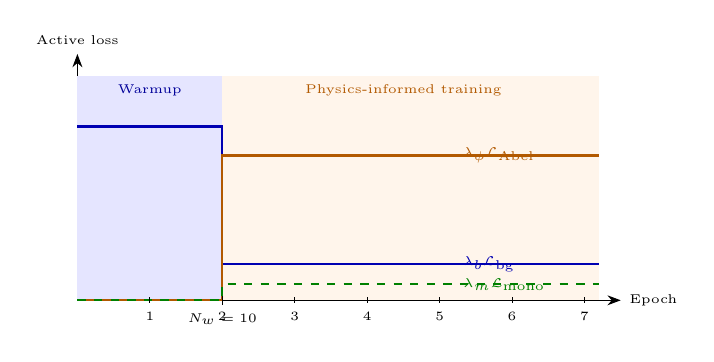
\begin{tikzpicture}[>=Stealth,every node/.style={font=\tiny},
                    scale=0.92,transform shape]
\draw[->] (0,0) -- (7.5,0) node[right] {Epoch};
\draw[->] (0,0) -- (0,3.4) node[above,font=\tiny] {Active loss};
\fill[blue!10] (0,0) rectangle (2.0,3.1);
\fill[orange!8] (2.0,0) rectangle (7.2,3.1);
\node[text=blue!60!black] at (1.0,2.9) {Warmup};
\node[text=orange!70!black] at (4.5,2.9) {Physics-informed training};
\draw[thick,blue!70!black]   (0,2.4)--(2,2.4)--(2,0.5)--(7.2,0.5);
\node[right,text=blue!70!black] at (5.2,0.5) {$\lambda_b\mathcal{L}_\mathrm{bg}$};
\draw[thick,orange!70!black] (0,0)--(2,0)--(2,2.0)--(7.2,2.0);
\node[right,text=orange!70!black] at (5.2,2.0) {$\lambda_\phi\mathcal{L}_\mathrm{Abel}$};
\draw[thick,green!50!black,dashed] (0,0)--(2,0)--(2,0.22)--(7.2,0.22);
\node[right,text=green!50!black] at (5.2,0.22) {$\lambda_m\mathcal{L}_\mathrm{mono}$};
\draw (2,0.06)--(2,-0.06) node[below] {$N_w=10$};
\foreach \x in {1,2,3,4,5,6,7}
  \draw (\x,0.04)--(\x,-0.04) node[below] {\x};
\end{tikzpicture}

\column{0.48\textwidth}
\begin{block}{The Ne$\to$0 collapse problem}
  \scriptsize
  At random init: $N(h)\!\approx\!0$\\
  $\Rightarrow h'_\mathrm{pred}\!\approx\!511\,\mathrm{km}$ (top of grid)\\
  $h'_\mathrm{obs}\!\approx\!200$--$400\,\mathrm{km}$\\[3pt]
  Forward Abel gradient pushes $N$ further toward 0.\\[3pt]
  \textbf{Warmup fix}: bg loss first teaches a\\
  non-trivial $N(h)$ shape from IRI prior;\\
  Abel inversion then corrects physics consistency.\\[3pt]
  \textbf{Ramp}: $\lambda_\phi$ increases linearly from 0\\
  to $10^{-4}$ over 10 post-warmup epochs.
\end{block}
\vspace{3pt}
\begin{exampleblock}{Stage 2 (real data)}
  \scriptsize
  No background term ($\lambda_b\!=\!0$)\\
  Physics-only: Abel inversion + monotone\\
  Optional: freeze FiLM generator\\
  $\Rightarrow$ preserves Stage 1 geophysical prior
\end{exampleblock}
\end{columns}
\end{frame}

% =================================================================
\section{Training Results \& Validation}
% =================================================================

\begin{frame}{Stage-1 Training: Loss Convergence}
\begin{columns}
\column{0.50\textwidth}
\scriptsize
\textbf{Warmup run (bg-only, 5 shards):}
\begin{tabular}{lrrrr}
\toprule
Ep & Train bg & Val bg & Train Abel & LR\\
\midrule
0 & $8.5\times10^{-4}$ & $4.0\times10^{-5}$ & 0.0 & $3.0\times10^{-4}$ \\
1 & $5.3\times10^{-5}$ & $2.5\times10^{-5}$ & 0.0 & $2.99\times10^{-4}$ \\
2 & $4.0\times10^{-5}$ & $2.5\times10^{-5}$ & 0.0 & $2.98\times10^{-4}$ \\
3 & $3.2\times10^{-5}$ & $1.5\times10^{-5}$ & 0.0 & $2.97\times10^{-4}$ \\
4 & $2.5\times10^{-5}$ & $8.4\times10^{-6}$ & 0.0 & $2.95\times10^{-4}$ \\
\bottomrule
\end{tabular}
\vspace{3pt}
\begin{itemize}\tiny
  \item Abel = 0 during warmup ($N_w = 10$ epochs)
  \item Val bg already $\mathcal{O}(10^{-5})$ after 4 epochs
  \item BG loss converges rapidly in log-norm Ne space
  \item Abel inversion ramp begins after warmup
  \item Full run: 270 shards, 50--100 epochs on VEGA
\end{itemize}

\column{0.47\textwidth}
\begin{block}{\scriptsize Component breakdown (Abel inversion path)}
  \scriptsize
  \begin{tabular}{lrl}
  \toprule
  Term & Target & Notes \\
  \midrule
  $\mathcal{L}_\mathrm{bg}$   & $<10^{-4}$ & log-norm MSE \\
  $\mathcal{L}_\mathrm{Abel}$ & $<0.05$    & log$_{10}$ MSE \\
  $\mathcal{L}_\mathrm{mono}$ & $\to 0$    & topside only \\
  \midrule
  Abel $\lambda$ & $10^{-4}$ & ramped \\
  Warmup & 10 ep & bg-only \\
  Ramp & 10 ep & $0\to\lambda_\phi$ \\
  \bottomrule
  \end{tabular}
\end{block}
\vspace{3pt}
\begin{alertblock}{\scriptsize Full run (VEGA HPC)}
  \scriptsize
  \textbf{Data}: 270 shards (PBS array, \texttt{--shard 0-269})\\
  \textbf{Train}: 50--100 epochs on V100/A100 GPU node\\
  \textbf{Arch}: 1.43 M params; spatial-latent encoder
\end{alertblock}
\end{columns}
\end{frame}

\begin{frame}{Validation: Inference Test (3-Panel Diagnostic)}
\vspace{-0.1cm}
\begin{columns}
\column{0.36\textwidth}
\begin{center}
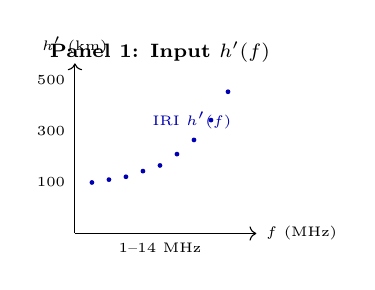
\begin{tikzpicture}[scale=0.72,every node/.style={font=\tiny}]
% Panel 1: input ionogram trace
\draw[->] (0,0)--(3.2,0) node[right] {$f$ (MHz)};
\draw[->] (0,0)--(0,3.0) node[above] {$h'$ (km)};
\node at (1.5,3.2) {\scriptsize\textbf{Panel 1: Input $h'(f)$}};
% draw dots simulating virtual height trace (increasing)
\foreach \x/\y in {0.3/0.9, 0.6/0.95, 0.9/1.0, 1.2/1.1,
                   1.5/1.2, 1.8/1.4, 2.1/1.65, 2.4/2.0,
                   2.7/2.5}{
  \fill[blue!70!black] (\x,\y) circle (1.2pt);
}
\node[blue!70!black,right] at (1.2,2.0) {IRI $h'(f)$};
% axis labels
\node[left] at (0,0.9) {100};
\node[left] at (0,1.8) {300};
\node[left] at (0,2.7) {500};
\node[below] at (1.5,0) {1--14 MHz};
\end{tikzpicture}
\end{center}

\column{0.36\textwidth}
\begin{center}
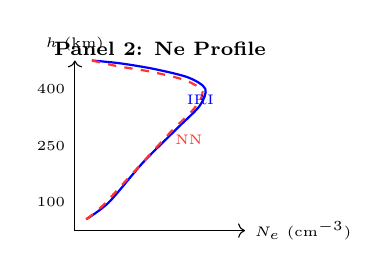
\begin{tikzpicture}[scale=0.72,every node/.style={font=\tiny}]
% Panel 2: Ne profiles
\draw[->] (0,0)--(3.0,0) node[right] {$N_e$ (cm$^{-3}$)};
\draw[->] (0,0)--(0,3.0) node[above] {$h$ (km)};
\node at (1.5,3.2) {\scriptsize\textbf{Panel 2: Ne Profile}};
% IRI profile (blue solid) — Chapman-like
\draw[blue,thick] plot[smooth] coordinates
  {(0.2,0.2)(0.6,0.5)(1.2,1.2)(1.8,1.8)(2.2,2.2)
   (2.3,2.5)(2.0,2.7)(1.4,2.85)(0.8,2.95)(0.3,3.0)};
% NN predicted (red dashed)
\draw[red!80,thick,dashed] plot[smooth] coordinates
  {(0.2,0.2)(0.5,0.45)(1.1,1.1)(1.7,1.75)(2.1,2.15)
   (2.25,2.45)(1.95,2.65)(1.35,2.8)(0.75,2.9)(0.3,3.0)};
\node[blue,right] at (1.8,2.3) {IRI};
\node[red!80,right] at (1.6,1.6) {NN};
\node[left] at (0,0.5) {100};
\node[left] at (0,1.5) {250};
\node[left] at (0,2.5) {400};
\end{tikzpicture}
\end{center}

\column{0.28\textwidth}
\begin{center}
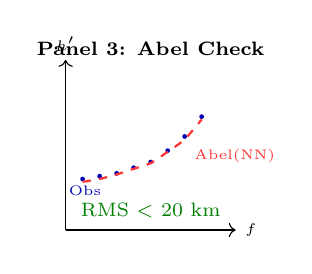
\begin{tikzpicture}[scale=0.72,every node/.style={font=\tiny}]
% Panel 3: Abel consistency
\draw[->] (0,0)--(3.0,0) node[right] {$f$};
\draw[->] (0,0)--(0,3.0) node[above] {$h'$};
\node at (1.5,3.2) {\scriptsize\textbf{Panel 3: Abel Check}};
\foreach \x/\y in {0.3/0.9, 0.6/0.95, 0.9/1.0, 1.2/1.1,
                   1.5/1.2, 1.8/1.4, 2.1/1.65, 2.4/2.0}{
  \fill[blue!70!black] (\x,\y) circle (1.2pt);
}
\draw[red!80,thick,dashed] plot[smooth] coordinates
  {(0.3,0.85)(0.6,0.9)(0.9,0.98)(1.2,1.08)
   (1.5,1.18)(1.8,1.38)(2.1,1.60)(2.4,1.95)};
\node[blue!70!black,left] at (0.8,0.7) {Obs};
\node[red!80,right] at (2.1,1.3) {Abel(NN)};
\node[font=\scriptsize,text=green!50!black] at (1.5,0.35)
  {RMS $<$ 20 km};
\end{tikzpicture}
\end{center}
\end{columns}

\vspace{2pt}
\begin{columns}
\column{0.33\textwidth}
  \begin{block}{\scriptsize Panel 1}
    \scriptsize
    \textbf{Input}: IRI-generated $h'(f)$\\
    Masked above foF2 (no reflection)
  \end{block}
\column{0.33\textwidth}
  \begin{block}{\scriptsize Panel 2}
    \scriptsize
    \textbf{Target}: IRI $N_e(h)$ (blue)\\
    \textbf{Predicted}: NN output (red dashed)
  \end{block}
\column{0.33\textwidth}
  \begin{exampleblock}{\scriptsize Panel 3}
    \scriptsize
    \textbf{Check}: Abel(NN) vs observed $h'(f)$\\
    Goal: RMS $<$20 km after 50 epochs
  \end{exampleblock}
\end{columns}
\end{frame}

% =================================================================
\section{Sporadic-E: Physics \& Extension}
% =================================================================

\begin{frame}{Sporadic-E: What It Is and Why It Matters}
\begin{columns}
\column{0.52\textwidth}
\begin{block}{What is Sporadic-E (Es)?}
  \small
  Thin layers ($\lesssim$1--2 km) of enhanced ionization at \textbf{90--130 km}
  altitude, composed predominantly of metallic ions (Fe$^+$, Mg$^+$, Na$^+$)
  from meteor ablation.\\[4pt]
  \textbf{Key signatures on ionograms:}
  \begin{itemize}\scriptsize
    \item Flat trace at low virtual heights ($\sim$100--120 km)
    \item High echo intensity at 1--5 MHz
    \item \textbf{Blanketing Es} (EsB): reflects \emph{all} HF — masks F layer
    \item \textbf{Transparent Es}: partial propagation — dual echoes
  \end{itemize}
\end{block}
\vspace{3pt}
\begin{alertblock}{Impact on NN-POLAN}
  \scriptsize
  IRI does \emph{not} model Es $\Rightarrow$ synthetic training data has no Es\\
  Blanketing Es: $h'(f)$ shows E-layer reflection, not F-layer\\
  Model may invert the wrong layer — need Es detection first
\end{alertblock}

\column{0.44\textwidth}
\begin{block}{Formation physics}
  \small
  \textbf{1. Meteor ablation} (ion source):\\
  \quad $\sim$100 tonnes/day of meteoric material\\
  \quad ablates at 80--120 km, deposits Fe, Mg, Na\\[4pt]
  \textbf{2. Wind-shear convergence} (primary mechanism):\\
  \quad Tidal and gravity waves create horizontal\\
  \quad wind shear $\partial u/\partial z$ at $\sim$100 km\\
  \quad $\Rightarrow$ \textbf{convergent ion motion} compresses\\
  \quad metallic ions into thin layers\\[4pt]
  \textbf{3. E$\times$B drift} (electric field modulation):\\
  \quad Polarization electric fields from neutral\\
  \quad wind dynamo enhance/suppress Es\\[4pt]
  \textbf{Diurnal pattern}: peaks in summer daytime\\
  \quad midlatitudes (strongest tidal wind shear)
\end{block}
\end{columns}
\end{frame}

\begin{frame}{Sporadic-E: Ionogram Morphology \& NN Extension Plan}
\begin{columns}
\column{0.46\textwidth}
\begin{center}
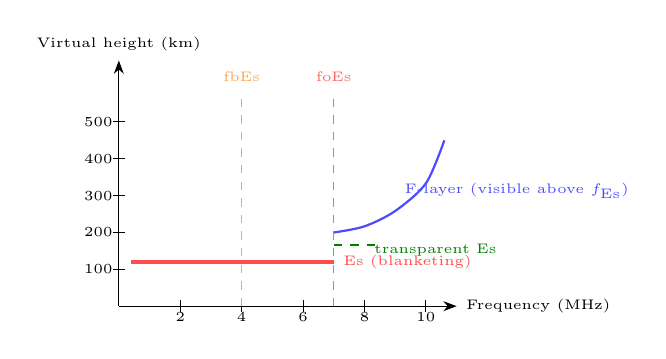
\begin{tikzpicture}[>=Stealth,scale=0.78,every node/.style={font=\tiny}]
\draw[->] (0,0)--(5.5,0) node[right] {Frequency (MHz)};
\draw[->] (0,0)--(0,4.0) node[above] {Virtual height (km)};

% axis ticks
\foreach \y/\lbl in {0.6/100, 1.2/200, 1.8/300, 2.4/400, 3.0/500}
  \draw (-0.1,\y)--(0.1,\y) node[left=1pt] {\lbl};
\foreach \x/\lbl in {1/2, 2/4, 3/6, 4/8, 5/10}
  \draw (\x,-0.1)--(\x,0.1) node[below=1pt] {\lbl};

% Es trace (flat, ~120 km)
\draw[red!70,very thick] (0.2,0.72) -- (3.5,0.72);
\node[red!70,right] at (3.5,0.72) {Es (blanketing)};

% F-layer trace (above fEs)
\draw[blue!70,thick] plot[smooth] coordinates
  {(3.5,1.2)(4.0,1.3)(4.5,1.55)(5.0,2.0)(5.3,2.7)};
\node[blue!70,above right] at (4.5,1.6) {F-layer (visible above $f_\mathrm{Es}$)};

% Es transparent window
\draw[green!50!black,dashed,thick] (3.5,1.0) -- (4.2,1.0);
\node[green!50!black,right] at (4.0,0.92) {transparent Es};

% foEs marker
\draw[red!60,dashed] (3.5,0) -- (3.5,3.5);
\node[red!60,above] at (3.5,3.5) {foEs};

% fblEs marker
\draw[orange!70,dashed] (2.0,0) -- (2.0,3.5);
\node[orange!70,above] at (2.0,3.5) {fbEs};

\end{tikzpicture}
\end{center}

\column{0.50\textwidth}
\begin{block}{Types of Es on ionograms}
  \scriptsize
  \begin{tabular}{@{}lp{5cm}@{}}
  \toprule
  \textbf{Type} & \textbf{Description}\\
  \midrule
  \textbf{EsB} (blanketing) & Strong reflection; blocks F-layer echoes below foEs\\
  \textbf{EsT} (transparent) & Partial reflections; F-layer visible above fbEs\\
  \textbf{EsC} (cusp) & Isolated patches; retardation echoes\\
  \textbf{EsF} (flat) & Perfectly flat trace; ionosphere nearly homogeneous\\
  \bottomrule
  \end{tabular}
\end{block}
\vspace{4pt}
\begin{exampleblock}{Proposed NN-POLAN extension}
  \scriptsize
  \textbf{Step 1} — \textbf{Es Detector} (classification):\\
  \quad Binary CNN: Is Es present? What type?\\[3pt]
  \textbf{Step 2} — \textbf{Es-Aware Inversion}:\\
  \quad Add Es flag to conditioning vector $c$\\
  \quad Separate loss branch for E-layer peak\\[3pt]
  \textbf{Step 3} — \textbf{Es Synthetic Data}:\\
  \quad Augment PyIRI profiles with Chapman Es layer\\
  \quad Vary $h_\mathrm{Es}$, $N_{m\mathrm{Es}}$, half-thickness $\sim$1 km
\end{exampleblock}
\end{columns}
\end{frame}

% =================================================================
% \section{Codebase Overview}
% =================================================================

% \begin{frame}{Codebase Layout and Configuration}
% \begin{columns}
% \column{0.48\textwidth}
% \vspace{-0.1cm}
% \begin{tikzpicture}[>=Stealth,every node/.style={font=\tiny},
%                     scale=0.90,transform shape]
% \node[grbox,minimum width=5.2cm,minimum height=0.42cm,
%       fill=gray!8] (root) at (0,0)
%   {\texttt{nn\_inversion/}};

% \node[pbox,minimum width=2.4cm,below left=0.38cm and 0.3cm of root]
%   (fm)  {\texttt{forward\_model.py}\\Abel integral (numpy)};
% \node[pbox,minimum width=2.4cm,below right=0.38cm and 0.3cm of root]
%   (cfg) {\texttt{config.py}\\NNCfg $\leftarrow$ config.toml};

% \node[obox,minimum width=2.4cm,below=0.28cm of fm]
%   (arch) {\texttt{training/architecture.py}\\NNPolan (PyTorch)};
% \node[obox,minimum width=2.4cm,below=0.28cm of cfg]
%   (sd)   {\texttt{training/synthetic\_data.py}\\PyIRI + pyomnidata};

% \node[gbox,minimum width=2.4cm,below=0.28cm of arch]
%   (pl)   {\texttt{training/physics\_loss.py}\\Abel+mono+bg};
% \node[gbox,minimum width=2.4cm,below=0.28cm of sd]
%   (tr)   {\texttt{training/trainer\_stage1/2.py}\\Training loops};

% \node[ybox,minimum width=2.4cm,below=0.28cm of pl]
%   (net)  {\texttt{network.py}\\Pure-numpy inference};
% \node[ybox,minimum width=2.4cm,below=0.28cm of tr]
%   (exp)  {\texttt{training/export\_weights.py}\\.pt $\to$ .npz};

% \draw[arr] (root)--(fm); \draw[arr] (root)--(cfg);
% \draw[arr] (cfg)--(arch); \draw[arr] (cfg)--(sd);
% \draw[arr] (cfg)--(pl); \draw[arr] (cfg)--(tr);
% \end{tikzpicture}

% \column{0.49\textwidth}
% \begin{block}{\scriptsize Single source of truth: \texttt{config.toml}}
%   \tiny
%   \texttt{[nn\_inversion.forward\_model]} — grids, $f_p^2$ const\\
%   \texttt{[nn\_inversion.data]} — lat/lon/year/DOY/UT steps\\
%   \texttt{[nn\_inversion.quality]} — foF2 bounds, min freqs\\
%   \texttt{[nn\_inversion.model]} — latent/feat/film dims\\
%   \texttt{[nn\_inversion.normalisation]} — $\mu,\sigma$ for all inputs\\
%   \texttt{[nn\_inversion.training]} — epochs, LR, $\lambda$s\\[3pt]
%   \textbf{All logging}: \texttt{loguru} (unified across codebase)\\
%   \textbf{Dead imports}: removed; \textbf{iricore}: replaced by PyIRI
% \end{block}
% \vspace{2pt}
% \begin{exampleblock}{\scriptsize Quick-start}
%   \tiny
%   \texttt{\# 1. Generate shard}\\
%   \texttt{python synthetic\_data.py --shard 0 --n\_shards 270 \\
%     \;\;--out\_dir /tmp/polan}\\[2pt]
%   \texttt{\# 2. Train (Stage 1)}\\
%   \texttt{python trainer\_stage1.py --data\_dir /tmp/polan \\
%     \;\;--out\_dir /tmp/out --epochs 50}\\[2pt]
%   \texttt{\# 3. Test inference}\\
%   \texttt{python test\_inference.py --ckpt /tmp/out/best.pt \\
%     \;\;--sample 42}\\[2pt]
%   \texttt{\# 4. Export weights}\\
%   \texttt{python export\_weights.py --ckpt best.pt --out WI937.npz}
% \end{exampleblock}
% \end{columns}
% \end{frame}

% =================================================================
\section{Next Steps}
% =================================================================

\begin{frame}{Roadmap}
\begin{columns}
\column{0.48\textwidth}
\begin{block}{Stage 1 — Foundation model}
  \scriptsize
  \begin{itemize}
    \item[$\checkmark$] FiLM encoder-decoder; \textbf{spatial-latent} (flatten, not pool)
    \item[$\checkmark$] Synthetic data: PyIRI + OMNI (1995--2024)
    \item[$\checkmark$] \textbf{Abel inversion loss} (singularity-free, log$_{10}$ MSE)
    \item[$\checkmark$] Warmup+ramp curriculum; topside-only monotone
    \item[$\checkmark$] config.toml single source of truth; loguru logging
    \item[$\checkmark$] Convergence diagnostics (\texttt{diagnose\_convergence.py})
    \item[$\square$] \textbf{Full VEGA run}: 270 shards, 50--100 epochs
    \item[$\square$] \textbf{Validate}: log$_{10}$ Abel MSE $<$ 0.05; Ne shape
  \end{itemize}
\end{block}
\vspace{3pt}
\begin{block}{Stage 2 — Station assimilation}
  \scriptsize
  \begin{itemize}
    \item[$\checkmark$] Abel inversion loss path implemented (\texttt{trainer\_stage2.py})
    \item[$\square$] Fine-tune on WI937 RIQ traces (pending Stage 1 best.pt)
    \item[$\square$] Per-station \texttt{.npz} in \texttt{weights/} directory
    \item[$\square$] Zero-dependency inference via \texttt{network.py}
  \end{itemize}
\end{block}

\column{0.48\textwidth}
\begin{block}{Sporadic-E extension}
  \scriptsize
  \begin{itemize}
    \item[$\square$] Es detector: classify EsB / EsT / none
    \item[$\square$] Augment synthetic data with artificial Es layers
    \item[$\square$] Add Es flag/intensity to conditioning vector $c$
    \item[$\square$] E-layer peak loss branch ($h_\mathrm{Es}$, $N_{m\mathrm{Es}}$)
  \end{itemize}
\end{block}
\vspace{3pt}
\begin{alertblock}{Open questions}
  \scriptsize
  \begin{itemize}
    \item How many real ionograms for Stage 2?\\
          ($\sim$500 clean traces/station is working estimate)
    \item CuPy for Abel GPU path? (installed, pending)
    \item Dual-polarisation (O-mode + X-mode) as input?
    \item Stage 2 convergence criterion?
  \end{itemize}
\end{alertblock}
\vspace{3pt}
\begin{exampleblock}{Longer-term}
  \tiny
  Ensemble UQ\quad|\quad
  hmF2/foF2 head\quad|\quad
  Real-time API\quad|\quad
  \textit{JGR: ML} manuscript
\end{exampleblock}
\end{columns}
\end{frame}

% =================================================================
\begin{frame}{Summary}
% =================================================================
\begin{center}
\large\textbf{NN-POLAN: Where We Stand}
\end{center}
\vspace{2pt}
\begin{columns}
\column{0.24\textwidth}
\begin{block}{\centering\scriptsize Physics}
  \centering\scriptsize
  Abel integral as core supervision — not just post-hoc
\end{block}
\column{0.24\textwidth}
\begin{block}{\centering\scriptsize Data}
  \centering\scriptsize
  30-yr IRI library with real F10.7/Kp from OMNI
\end{block}
\column{0.24\textwidth}
\begin{block}{\centering\scriptsize Architecture}
  \centering\scriptsize
  FiLM conditioning: one model, all geophysical contexts
\end{block}
\column{0.24\textwidth}
\begin{block}{\centering\scriptsize Es Extension}
  \centering\scriptsize
  Sporadic-E detector + Es-aware conditioning planned
\end{block}
\end{columns}
\vspace{5pt}
\begin{columns}
\column{0.49\textwidth}
\begin{alertblock}{\centering\scriptsize Key engineering fixes}
  \scriptsize
  \begin{itemize}
    \item \textbf{Flatten bottleneck}: pool $\to$ flatten preserves\\
          freq-position $\to$ Abel gradients can propagate
    \item \textbf{Abel inversion loss}: singularity removed from graph\\
          log$_{10}$-MSE vs $N_\mathrm{abel}$ on bottomside only
    \item Warmup $+$ ramp curriculum $\to$ no Ne collapse
    \item Topside-only monotone (not full profile)
    \item Full \texttt{config.toml} consolidation; loguru logging
    \item Convergence diagnostics: 4-config gradient health check
  \end{itemize}
\end{alertblock}
\column{0.49\textwidth}
\begin{exampleblock}{\centering\scriptsize Immediate action items}
  \scriptsize
  \begin{enumerate}
    \item Submit 270-shard PBS array on VEGA (Stage 1)
    \item Train 50--100 epochs; monitor Abel log$_{10}$ MSE
    \item Validate inference: \texttt{test\_inference.py} 3-panel check
    \item Begin Stage 2 data prep (WI937 RIQ files)
    \item Update whitepaper \& slides (in progress)
    \item Prototype Es extension (future v2.0)
  \end{enumerate}
\end{exampleblock}
\end{columns}
\end{frame}

% =================================================================
\begin{frame}[plain]
  \begin{center}
    \vspace{1.5cm}
    {\LARGE \textbf{Thank you}}\\[12pt]
    {\large Questions \& Discussion}\\[20pt]
    \small
    Code: \href{https://github.com/shibaji7/pynasonde}{\texttt{github.com/shibaji7/pynasonde}}\\[4pt]
    Module: \texttt{pynasonde.vipir.analysis.nn\_inversion}\\[4pt]
    Config: \texttt{pynasonde/config.toml} $\to$ \texttt{[nn\_inversion.*]}
  \end{center}
\end{frame}

\end{document}
